\documentclass[a4paper]{article}
\usepackage{fancyhdr}
\usepackage[pdftex]{graphicx}
\usepackage{sidecap}
\usepackage{listings}
\usepackage{color}
\usepackage[export]{adjustbox}
\usepackage{subcaption}
\usepackage{graphicx}

\usepackage{hyperref}
\hypersetup{
    colorlinks=true,
    linkcolor=blue,
    filecolor=magenta, 
    urlcolor=cyan,
    bookmarks=true,
    pdfpagemode=FullScreen,
}
\usepackage{geometry}
 \geometry{
 a4paper,
 total={210mm,297mm},
 left=15mm,
 right=15mm,
 top=15mm,
 bottom=15mm,
 }

\usepackage{glossaries}


\makeglossaries
\newglossaryentry{FSM}
{
    name=FSM,
    description={Finite State Machine}
}

\definecolor{mygreen}{RGB}{25,172,0} % color values Red, Green, Blue
\definecolor{mylilas}{RGB}{170,55,241}
\definecolor{dkgreen}{rgb}{0,0.6,0}
\definecolor{gray}{rgb}{0.5,0.5,0.5}
\definecolor{mauve}{rgb}{0.58,0,0.82}

\pagestyle{fancy}
\fancyhf{}
\rhead{Vangjush Komini}
\lhead{KU Leuven}
\rfoot{Page \thepage}
\lfoot{Simulation of 2D array in field II}


\lstset{inputpath=Code}
\graphicspath{{Images/}}





\begin{titlepage}

\title{Simulation of 2D array in field II}

\author{
\href{mailto:vangjush.komini@uzleuven.be}{Vangjush Komini}\\ 
}
\end{titlepage}






\begin{document}


\maketitle


A 2D ultrasound arrays has been simulated in field II. A fully wired configuration has been compared with another configuration where consequently 1 after 3 crystals has been wired.
The pressure field on transmit has been compared for these two both simulation for 4 different focusing points. In the figure \ref{1} there are two columns of different results. On the left hand side the the proposed configuration with its transmit pressure field whereas on the right hand side there is the fully wired system and its transmit pressure field on four different focusing points.
In figure \ref{2} and \ref{3} are the visualization of the partially wired and fully wired phase.

Moving on the figure \ref{4}  and \ref{5} the pressure field for the central point ($\phi=0$,$\theta=0$) are presented. In case of partially wired phase array \ref{4} there is not big concentration of the energy at the center. It is rather spread over a region of interest where the center of the region is the point of interest. On the other hand,  for the fully wired configuration the point of interest acquires big concentration \ref{5} of the energy contrary to the other configuration.

When the focus is elevated up with only \textbf{37.5 deg}  ($\phi=0$,$\theta=37.5$) there are side lobes in both configuration however in the partially wired system there is are more pronounced side-lobes on the lower side and on the upper left side of the pressure field. This imperfection will decay the resolution of the system. 

In case of a focus with a azimuth angle of \textbf{37.5 deg} ($\phi=37.5$,$\theta=0$) there are almost no side lobes for the fully wired configuration \ref{9} whereas the partially wired proposed configuration has a significantly high level of side lobes \ref{8} which it will of course decays the resolution of this point measurement. 


However to see even more the impact of the partially wired configuration \ref{1} the focus point has been elevated up with \textbf{37.5 deg} on an azimuth angle of \textbf{37.5 deg} ($\phi=37.5$,$\theta=37.5$). The pressure field for the fully wired phase array exhibit side lobes on its upper right side. Further more for the partialy wired array, the side lobes are prevalent not only at the upper side but even at the left center side of the preassure profile. 

\begin{figure}[!htbp]
\minipage{.5\textwidth}%
\centering
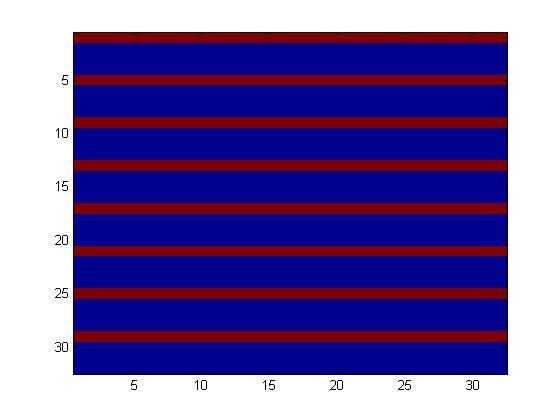
\includegraphics[width=.7\textwidth]{1.jpg}\\
\subcaption{}\label{2}
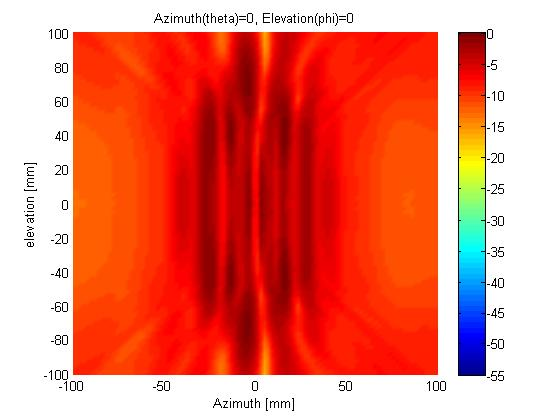
\includegraphics[width=.7\textwidth]{2.jpg}\\
\subcaption{}\label{4}
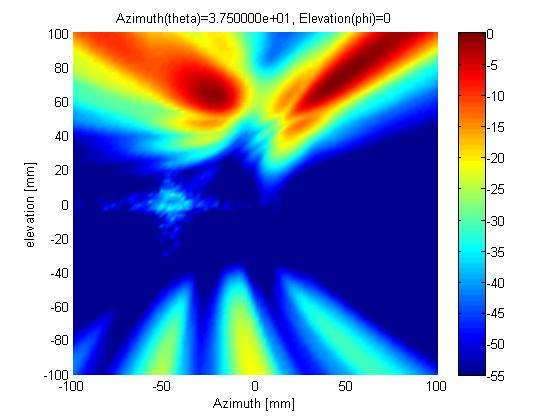
\includegraphics[width=.7\textwidth]{3.jpg}\\
\subcaption{}\label{6}
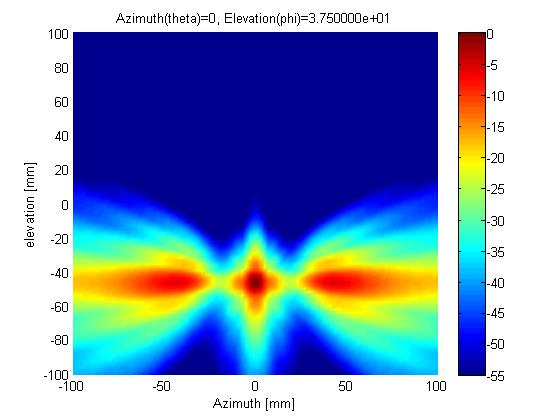
\includegraphics[width=.7\textwidth]{4.jpg}\\
\subcaption{}\label{8}
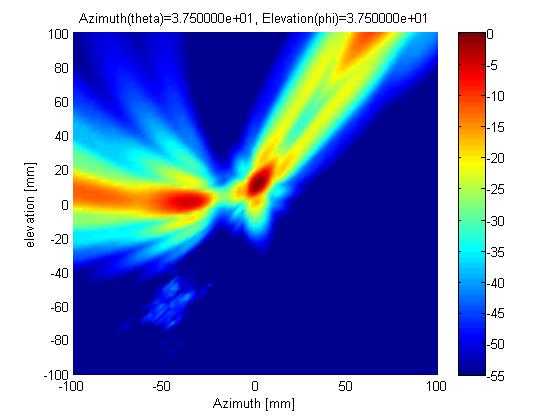
\includegraphics[width=.7\textwidth]{5.jpg}
\subcaption{}\label{10}
\endminipage\hfill
\minipage{.5\textwidth}%
\centering
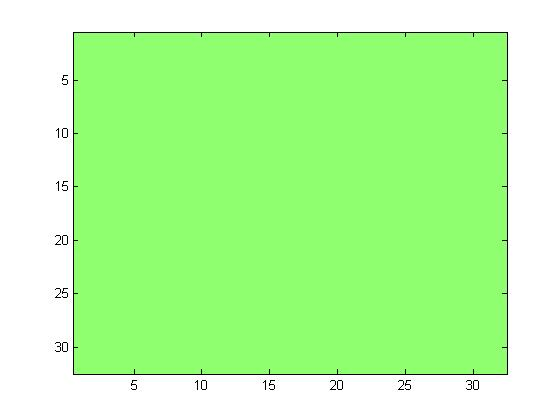
\includegraphics[width=.7\textwidth]{6.jpg}\\
\subcaption{}\label{3}
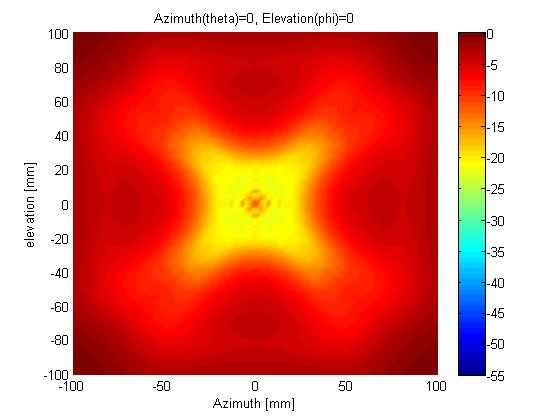
\includegraphics[width=.7\textwidth]{7.jpg}\\
\subcaption{}\label{5}
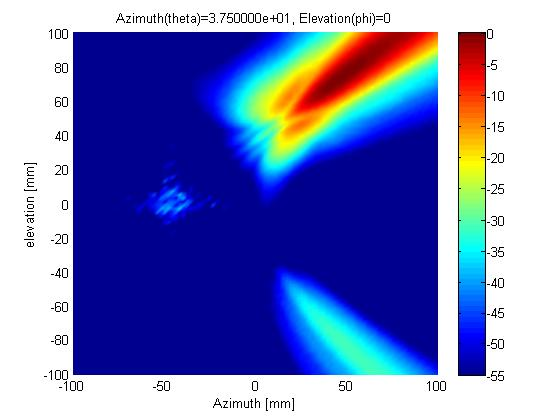
\includegraphics[width=.7\textwidth]{8.jpg}\\
\subcaption{}\label{7}
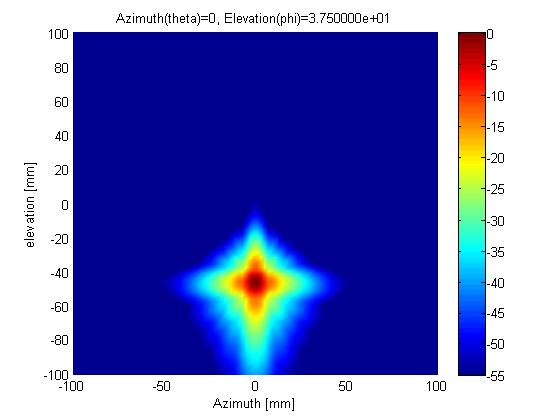
\includegraphics[width=.7\textwidth]{9.jpg}\\
\subcaption{}\label{9}
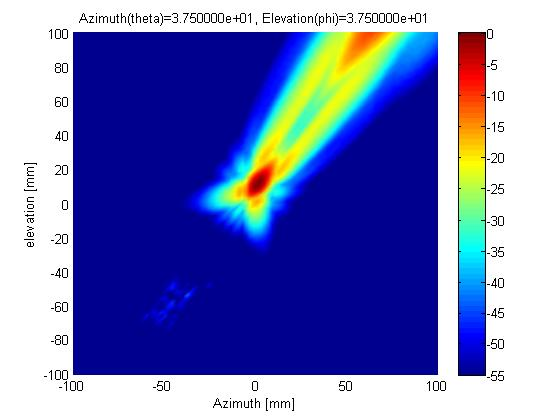
\includegraphics[width=.7\textwidth]{10.jpg}
\subcaption{}\label{11}
\endminipage\hfill
\caption{}\label{1}
\end{figure}




\lstset{language=Matlab,%
    %basicstyle=\color{red},
    breaklines=true,%
    morekeywords={matlab2tikz},
    keywordstyle=\color{blue},%
    morekeywords=[2]{1}, keywordstyle=[2]{\color{black}},
    identifierstyle=\color{black},%
    stringstyle=\color{mylilas},
    commentstyle=\color{mygreen},%
    showstringspaces=false,%without this there will be a symbol in the places where there is a space
    numbers=left,%
    numberstyle={\tiny \color{black}},% size of the numbers
    numbersep=9pt, % this defines how far the numbers are from the text
    emph=[1]{for,end,break},emphstyle=[1]\color{red}, %some words to emphasise
    %emph=[2]{word1,word2}, emphstyle=[2]{style},    
}

\newpage
\section{Main code}
\lstinputlisting{CarolinaExercise.m}





\end{document}

